\clearpage
Blank
\clearpage

\section{Introduction}

\subsection{Motivation}

In the age of digital documents, an author of content is confronted with the
question which document format to choose. Since every document format has its
advantages, one might not want to commit to a specific format to soon.

A series of blog posts might turn into a book or at least a pretty typeset
\emph{pdf}. An author also might want to give the reader the freedom to read
their text on different digital devices—e.g. mobile phones, tablets and
e-readers.

Luckily the problem of decoupling the initial document from output seems to be
solved by the rise of markup languages such as Markdown and the like. These
types of documents can be easily compiled into all sorts of output formats by
programs such as \emph{Pandoc} \cite{pandoc}.

If the reader has no objections to such a publishing system, they might read no
further and write away their next \emph{format-agnostic} document. But if they
are interested in how they can easily extend the syntax of their document and
let a type-checker reason about the \emph{well-formedness} of it, they may find
the findings gathered in this paper worth while.

\subsection{Type-safe extensibility}

This paper mostly outlines the ideas of the work on \emph{HSXML: Typed SXML}
\cite{hsxml} and its underlying approach of \emph{tagless-final style}
\cite{finally-tagless, finally-tagless-tut}.\\
The \emph{tagless-final style} is a solution to the expression problem
\cite{expression-problem}. It is closely related to the problem at hand, in that
it is concerned with the simultaneous extension of syntactic \emph{variants} and
interpretations of them—we call those \emph{observations}. This can be seen as
an extensibility in two dimensions. For those unfamiliar with the the expression
problem—section \ref{section_ep} provides an introduction.

\subsection{?}

In short a \emph{tagless-final encoded} representation of documents like
\emph{HSXML} has in our opinion two major advantages over markup languages such
as Pandoc’s internal one:

\begin{enumerate}
\item Guarantee the well-formedness of the document by construction
\item Easy and full extensibility without loosing the guarantees of 1.
\end{enumerate}

While having these two advantages we still do not want to loose perspective and
solve to our initial goal:

\begin{enumerate}
\item Writing documents that are format agnostic—i.e. observe our source in
different ways
\end{enumerate}

or as described in the Wikipedia-article on \emph{Markup Languages}

\begin{quote}
Descriptive markup

Markup is used to label parts of the document rather than to provide specific
instructions as to how they should be processed. Well-known examples include
\LaTeX{}, HTML, and XML. The objective is to decouple the inherent structure of
the document from any particular treatment or rendition of it. Such markup is
often described as "semantic".
\end{quote}

\clearpage

\section{Background: The Expression Problem} \label{section_ep}

The following description of the expression problem is short and precise and
stems from Zenger’s and Odersky’s paper \emph{Indepently Extensible Solutions to
  the Expression Problem} \cite{indie_solutions}.

\begin{quote}
  Since software evolves over time, it is essential for software systems to be
  extensible. But the development of extensible software poses many design and
  implementation problems, especially if extensions cannot be anticipated. The
  \emph{expression problem} is probably the most fundamental one among these
  problems. It arises when recursively defined datatypes and operations on
  these types have to be extended simultaneously.
\end{quote}

In this paper we call those \say{datatypes} \say{data variants} or in short
\say{variants} and the operations on them are called \say{observations}. This is
inspired by \emph{Extensibility for the Masses} \cite{object_algebra}.

To get a better intuition on what the expression problem is really concerned
with, we will introduce a small extensibility problem and explain the meaning of
these \emph{mystical dimensions} with its help:

The task is to find an easily extensible representation of \emph{algebraic
  expressions}—like e.g. $2+4-3$—in Haskell. We will present three different
encodings and discuss what kinds of extensibility they allow.

\subsection{ADT encoding}

When encoding algebraic expressions in \emph{algebraic data type (ADT)
  encoding}, we could write this definition:

\begin{lstlisting}
data Expr
  = Lit Int
  | Add Expr Expr
\end{lstlisting}

With the above code we defined two data variants, \texttt{Lit} and
\texttt{Add}. Now we can write multiple observations on those variants
easily:

\begin{lstlisting} 
eval :: Expr -> Int
eval (Lit i)   = i
eval (Add l r) = eval l + eval r

pretty :: Expr -> String
pretty (Lit i)   = show i
pretty (Add l r) =
     "(" ++ pretty l ++ ")"
  ++ "+"
  ++ "(" ++ pretty r ++ ")"
\end{lstlisting}

We assess that the ADT encoding is extensible in the dimension of observations.

If we wanted to add another variant—e.g. one for negation—we would have to
change not only the ADT definition but also all observations. This might be
feasible as long as we feel comfortable with changing the original code. But as
soon as someone else wrote observations depending on the original set of
variants, we risk breaking compatibility.

\subsection{OO encoding}
If we wanted to ensure that our representation is extensible in the dimension of
data variants, we could choose the \emph{object oriented (OO) encoding}. This
encoding is centered around the record type \texttt{ExprOO} with the following
definition:
\begin{lstlisting}
data ExprOO = ExprOO { evalThis   :: Int
                     , prettyThis :: String}
\end{lstlisting}

This definition states: an \texttt{Expr} is a value that can be evaluated to
both an \texttt{Int} and a \texttt{String}. Based on this we can create a set of
constructors.

\begin{lstlisting}
newLit :: Int -> ExprOO
newLit i = ExprOO i (show i)

newAdd :: ExprOO -> ExprOO -> ExprOO
newAdd l r = ExprOO evalResult prettyResult
 where
  evalResult   = evalThis l + evalThis r
  prettyResult =
       "(" ++ prettyThis l ++ ")"
    ++ "+"
    ++ "(" ++ prettyThis r ++ ")"
\end{lstlisting}

This set of data variants can now be easily extended. In the following we define
a constructor representing the algebraic operation of \emph{negation}.

\begin{lstlisting}
newNeg :: ExprOO -> ExprOO
newNeg e = ExprOO (- evalThis e) ("- " ++ prettyThis e)
\end{lstlisting}

These constructors can be used like the constructors of the ADT encoding to
create ASTs.

\begin{lstlisting}
exOO :: ExprOO
exOO = newAdd (newLit 4) (newNeg (newLit 2))
\end{lstlisting}
\begin{lstlisting}
> evalThis exOO
2
\end{lstlisting}

Although this representation is extensible in the dimension of data variants,
the set of observations is fixed by the definition of the \texttt{ExprOO} type.

\subsection{Church/Böhm-Berarducci encoding}
\label{subsection_BB_encoding}

Finally we will choose \emph{Böhm-Berarducci (BB) encoding} for our
representation which is the foundation of the tagless-final style.

Böhm and Berarducci used a technique, that is similar to Church encoding, to
show that ADTs can be represented by using solely using function application and
abstraction in \emph{System F} (i.e. polymorphic lambda-calculus)
\cite{boehm_berarducci}.

In practice this means that we could define lists, instead of using an ADT, the
following way:

\begin{lstlisting}
bbList :: (Int -> a -> a) -> a -> a
bbList cons nil = cons 2 (cons 1 nil)
\end{lstlisting}

To paraphrase the code: if we are supplied one interpretation for the
\texttt{nil} variant and one interpretation for the \texttt{cons} variant—that
takes one \texttt{Int} and the already evaluated rest of the list—we can
interpret the whole list.

We can generalize this idea: To evaluate an AST to a type $a$, we need to know
for each node type, how to evaluate it to $a$. If all these needed
\emph{evaluation strategies} are supplied, we can evaluate (i.e. \emph{fold})
the AST from the leaves up. These \emph{evaluation strategies} are called
\textbf{algebras}.\\
This is in essence the idea of Church/Böhm-Berarducci encoding.

In the appendix we include representation that is purely using application and
abstraction for our running example. But in Haskell we are luckily not
restricted to the features of lambda calculus. Therefore we can use record types
for storing \emph{algebras} (i.e. evaluation strategies).

Our algebras are of the following type:

\begin{lstlisting}
data ExprBP a = ExprBP { lit :: Int -> a
                       , add :: (a -> a -> a) }
\end{lstlisting}

The field called \texttt{lit} contains the interpretation for the leaves and
therefore is a function that evaluates an \texttt{Int} to some type \texttt{a}.
The \texttt{add} function takes two evaluated subtrees as an input—in form of
two \texttt{a}—and outputs also a value of type \texttt{a}.

An AST, using this definition, looks like this:

\begin{lstlisting}
exprBP :: ExprBP a -> a
exprBP (ExprBP lit add) = add (lit 4) (lit 2)
\end{lstlisting}

This is analogue to the BB encoded list from before, but, instead of getting
the algebras for \texttt{lit} and \texttt{add} one by one, the AST accepts one
algebra that bundles both.

\subsubsection{Writing algebras}

To evaluate those \emph{BB encoded} algebraic expressions, we have to define
algebras of the type \texttt{ExprBP}:

\begin{lstlisting}
evalExprBP :: ExprBP Int
evalExprBP = ExprBP evalInt evalAdd
  where
    evalInt i   = i
    evalAdd l r = l + r

prettyExprBP :: ExprBP String
prettyExprBP = ExprBP evalInt evalAdd
 where
  evalInt     = show
  evalAdd l r =
       "(" ++ l ++ ")"
    ++ "+"
    ++ "(" ++ r ++ ")"
\end{lstlisting}

\texttt{evalExprBP} can be defined even more concise in Haskell:

\begin{lstlisting}
evalExprBP :: ExprBP Int
evalExprBP = ExprBP id (+)
\end{lstlisting}

The AST from before, \texttt{exprBP}, can now be evaluated by supplying the
wanted algebra:

\begin{lstlisting}
> exprBP evalExprBP
6
> exprBP prettyExprBP
"(4)+(2)"
\end{lstlisting}

We can assess that we could define even more algebras this way and that this
encoding is therefore extensible in the dimension of algebras—i.e. observations.

\subsubsection{Add variants}

We have shown that the BB encoding is extensible in the dimension of
observations/algebras but the open question is how to define new variants.

This is can be done by defining a new data type for constructing algebras:

\begin{lstlisting}
data NegBP a = NegBP { neg :: a -> a }
\end{lstlisting}

Using this data type, we can define two new observations:

\begin{lstlisting}
evalNegBP :: NegBP Int
evalNegBP = NegBP (\e -> -e)

prettyNegBP :: NegBP String
prettyNegBP = NegBP (\e -> "-" ++ e)
\end{lstlisting}

Finally we are able to use \texttt{ExprBP} with \texttt{NegBP} in composition:

\begin{lstlisting}
mixedExpr :: ExprBP a -> NegBP a -> a
mixedExpr (ExprBP lit add) (NegBP neg) = add (lit 4) (neg (lit 2))
\end{lstlisting}
\begin{lstlisting}
> mixedExpr evalExprBP evalNegBP
2
\end{lstlisting}

Therefore the Böhm-Berarducci encoding is extensible in both dimensions.\\
If we wanted to add a new data variant, we would need to add a new data type
definition for creating corresponding algebras. And we can create new observers
by creating values of these data types (i.e. algebras).\\
As we have shown, these extensions also compose quite well in BB encoding.

Those familiar with the \say{Scrap your Boilerplate} pattern
\cite{scrap_type_classes} might notice that the \texttt{ExprBP} data type could
also be defined as a type class and the algebras—\texttt{evalExprBP} and
\texttt{prettyExprBP}—as instances of this type class. In section
\ref{section_tagless-final} we will demonstrate how the encoding with type
classes looks like.

%(Figure \ref{Expression_Problem})
%
%\vspace*{\fill}
%\begin{figure}
%    \centering
%    \includegraphics{resources/expression_problem_dimensions.png}
%\captionof{figure}{\label{Expression_Problem}
%Dimensions of the \emph{Expression Problem}}
%\end{figure}
%\vspace*{\fill}
\clearpage

\section{ADT encoded Markup}
\label{main_section}

In the last section we tried to find an extensible representation of
\emph{algebraic expressions}. Below we will examine how documents written in
markup languages like Markdown or \LaTeX{} can be represented.

We will have a look at the representation that Pandoc is using in this
section and then show in section \ref{section_tagless-final} how a
representation encoded in tagless-final style is an improvement over that.

\subsection{Pandoc's internals}

Pandoc is a program written in Haskell that parses a document in one format and
outputs the content in another format. It can for example create pdf documents
out of Markdown files with the help of \texttt{pdflatex}.

To translate the content of a document from one format to another, Pandoc first
parses the input into an abstract syntax tree (AST). As we have shown in section
\ref{section_ep} there a couple of encodings to choose from and Pandoc uses the
most common encoding: algebraic data types. In the following we will see what
this looks like in Haskell code.

A whole document with its meta data is in Pandoc defined as we would expect:

\begin{lstlisting}
data Pandoc = Pandoc Meta [Block]
\end{lstlisting}

The list of \texttt{Block} represents the content of the document.
\texttt{Block} is a sum type and has many cases. To get an understanding for
this encoding, it is sufficient to consider this subset:

\begin{lstlisting}
data Block
  = Paragraph   [Inline] -- ^ Paragraph
  | BulletList  [Block]  -- ^ Bullet list (list of items, each a block)
  | Heading Int [Inline] -- ^ Heading - level (int) and text (inlines)
\end{lstlisting}

The representation is therefore an ADT encoded rose tree. The \texttt{Block}
type is not only dependent on it self but also on \texttt{Inline}.
\texttt{Inline} represents all elements that can only appear inline in
documents. There are also quite many cases of this sum type and this is just
a subset of the original definition:

\begin{lstlisting}
data Inline
  = Str String      -- ^ Text (string)
  | Emph   [Inline] -- ^ Emphasized text (list of inlines)
  | Strong [Inline] -- ^ Strongly emphasized text (list of inlines)
\end{lstlisting}

The division of the AST cases into the sum types \texttt{Block} and
\texttt{Inline} puts a bit of a restriction on how those ASTs can be
constructed. This can be quite helpful when writing parsers and guarantees at
least of little bit of well-formedness. For example something like this cannot
be constructed due to the differentiation between \texttt{Block} and
\texttt{Inline}:

\begin{lstlisting}
> [ Heading 1  [ Heading 2 [Str "Headingception!!"]]]
<interactive>:25:14:
    Couldn't match expected type 'Inline' with actual type 'Block'
    In the expression: Heading 2 [Str "Headingception!!"]
    In the second argument of 'Heading' namely
      '[Heading 2 [Str "Headingception!!"]]'
\end{lstlisting}

Given the ADT encoded representation we can write observations that interpret
this data in different ways (Figure \ref{Pandoc_Views}). So in the dimension of
observations the ADT encoding is also in Pandoc’s case extensible.

We can construct a tree in the host language, Haskell, and interpret it in two
different ways:
\begin{lstlisting}
groceryList :: [Block]
groceryList
  = [ Heading 1  [ Str "Grocery list"]
    , BulletList [ Paragraph [ Str "1 Banana"]
                 , Paragraph [ Str "2 "
                             , Emph [Str "organic"]
                             , Str " Apples"]]]
\end{lstlisting}

\begin{lstlisting}
groceryListCM :: Markdown
groceryListCM = mconcatMap blockToCMark groceryList

groceryListLaTeX :: LaTeX
groceryListLaTeX = mconcatMap blockToLaTeX groceryList
\end{lstlisting}

We can make our life a bit easier by adding an instance for \texttt{IsString}
for our representation. This injects \texttt{String} automatically into our data
types by applying \texttt{fromString} to it.

\begin{lstlisting}
instance IsString Inline where
  fromString = Str
\end{lstlisting}


Our initial definition is now even more concise:

\begin{lstlisting}
groceryList :: [Block]
groceryList
  = [ Heading 1  [ "Grocery list"]
    , BulletList [ Paragraph [ "1 Banana"]
                 , Paragraph [ "2 " , Emph ["organic"] , " Apples"]]]
\end{lstlisting}

\begin{figure}
\begin{lstlisting}
newtype Markdown = Markdown String deriving (Monoid, IsString)
newtype LaTeX    = LaTeX    String deriving (Monoid, IsString)

blockToCMark :: Block -> Markdown
blockToCMark (Paragraph text)     = mconcatMap inlineToCMark text
blockToCMark (BulletList docs)    = ...
blockToCMark (Heading level text) = ...

inlineToCMark :: Inline -> Markdown
inlineToCMark (Str content)     = fromString content
inlineToCMARK (Emph contents)   =
            "*"
  `mappend` mconcatMap inlineToCMark contents
  `mappend` "*"
inlineToCMARK (Strong contents) = ...

blockToLaTeX :: Block -> LaTeX
...

inlineToLaTeX :: Inline -> LaTeX
...
\end{lstlisting}
\captionof{figure}{\label{Pandoc_Views}
Observations of Pandoc’s ADT encoding}
\end{figure}

\subsection{Extensibility Analysis}

The simple ADT encoding works very well as long as we have foreseen every
constructor we might want to create. But as soon as we want to add a new kind of
constructor—e.g. a node representing the em dash—we are out of luck. Even if we
have access to the original ADT-definition and we could add this new
constructor, this would break all existing observations that were written for
the original set of constructors.

As shown in subsection \ref{subsection_BB_encoding}, we can do better than this
using \emph{Böhm-Berarducci encoding}.

\clearpage

\section{Simple Tagless-Final Encoding} \label{section_tagless-final}

In subsection \ref{subsection_BB_encoding} we passed the algebras of the
\emph{Böhm-Berarducci encoding} explicitly. In the following we will use type
classes for the automatic passing of the algebra/observation dictionaries. Using
BB encoding with the help of type classes is called \emph{tagless-final style}
and was first described by Kiselyov, Carette and Chan in \emph{Finally Tagless,
  Partially Evaluated} \cite{finally-tagless}.

Our first attempt to encode our document in the tagless-final encoding will not
have the distinction between \texttt{Doc} and \texttt{Inline}—which was enforced
by the Pandoc-encoding. But later we will see that we are able to recover that
property quite easily with great extensibility properties.

The basic idea of the tagless-final encoding is to create a type class that
specifies all our variants in Böhm-Berarducci encoding. This is analogue to the
\emph{Scrap your type class} variant defined in section
\ref{subsection_BB_encoding}, with the only technical difference:\\
The observers/algebras are now specified with the help of type classes and the
implementations of these specifications are instances of this type class.

\subsection{Böhm-Berarducci encoding with type classes}

In Figure \ref{BB_encoded_AST} we can see that the type classes \texttt{Block}
and \texttt{Inline} look similar to the record types from the original BB
encoding. Compared to the ADT encoded variants, these are polymorphic in the
return type and former recursive fields are now also polymorphic.

These polymorphic parts of the signature consist not only of the type parameter
\texttt{a}. Instead \texttt{a} is wrapped in the \emph{newtype} \texttt{Doc}.
This has the following reason:\\
Our first tagless-final encoding could also be realized without this wrapper and
\texttt{Doc} is not of much use—\textbf{yet}. But \texttt{Doc} will be vital
later on when we add context awareness to our encoding.

\subsubsection{Constructing ASTs}

In contrast to the encoding in section \ref{subsection_BB_encoding}, algebras do
not need to be passed explicitly to the AST definitions. This leads to even more readable code:

\begin{lstlisting}
groceryList :: (Block a, Inline a) => [a]
groceryList
  = [ heading 1  [str "Grocery list"]
    , bulletList [ paragraph [ str "1 Banana"]]
                 , paragraph [ str "2 "
                             , emph [str "fresh"]
                             , str " Apples"] ]
\end{lstlisting}

The reader might notice that we cannot use the same carrier type for different
interpretations of our AST—otherwise we would get overlapping instances. This
can be quite easily solved by wrapping the carrier type into a \emph{newtype}
and add or derive the needed instances for it. In our case \texttt{Markdown} is
simply a \emph{newtype} of \texttt{String}. Therefore the instances for
\texttt{IsString} and \texttt{Monoid} are straightforward to implement and can
even be derived using GHC’s \texttt{GeneralizedNewtypeDeriving} language pragma.

Figure \ref{FT_Observer} shows the implementation of observers in the
tagless-final encoding. The implementation is really similar to the one in the
ADT encoding. If we have close look though, we can see one difference: since our
data type is Böhm-Berarducci encoded, the observations do not need to be called
recursively. This makes both our code simpler and is essential for
extensibility.

As before, we can automate the injection of \texttt{String} into our encoding by
using the \texttt{OverloadedStrings} language pragma. We do this be adding a
constraint on the type classes, so every output format (i.e. carrier type) must
have an \texttt{IsString} instance.

\begin{figure}
\begin{lstlisting}
newtype Doc doc = Doc doc

-- DocConstraint defined using ConstraintKinds
type DocConstraint doc = (Monoid doc, IsString doc)

instance DocConstraint doc => -- Have to restrict for the use of 'mempty'
  Monoid (Doc doc) where
  mappend (Doc doc1) (Doc doc2) = Doc $ doc1 `mappend` doc2
  mempty = Doc mempty

-- Algebra specification

class Block a where
  paragraph  ::        [Doc a] -> Doc a
  bulletList ::        [Doc a] -> Doc a
  heading    :: Int -> [Doc a] -> Doc a

class DocConstraint a =>
  Inline a where
  str    :: String -> Doc a
  str = Doc . fromString
\end{lstlisting}
\captionof{figure}{\label{BB_encoded_AST}
Böhm-Berarducci encoding using type classes—i.e. tagless-final style}
\end{figure}

\begin{figure}
\begin{lstlisting}
-- Implement Markdown observer

instance Block Markdown where
  paragraph = fromInline . mconcat
  bulletList = ...
  heading level = ...

instance Inline Markdown

instance Styles Markdown where
  emph   texts = "*"  `mappend` mconcat texts `mappend` "*"
  strong texts = ...


-- Implement LaTeX observer

instance Block LaTeX where
...

instance Inline LaTeX where
...

instance Styles LaTeX where
...
\end{lstlisting}
\captionof{figure}{\label{FT_Observer}
Observer implementation in the tagless-final encoding}
\end{figure}


Interestingly \texttt{Doc} has now no dependency on \texttt{Inline} anymore and
we are now allowed to create the following AST:

\begin{lstlisting}
badHeading = [ heading 1  [ heading 2 [str "Headingception!!"]]]
\end{lstlisting}

\subsection{Where tagless-final shines}

As noted above, we lost the distinction between \texttt{Doc} and
\texttt{Inline}. But we also gained something—\emph{Doc} can now be used
without \emph{Inline} and we can now also add new constructors without changing our
original constructor definitions:

\begin{lstlisting}
class Styles doc where
  emph   :: [DocWithCtx InlineCtx doc] -> DocWithCtx InlineCtx doc
  strong :: [DocWithCtx InlineCtx doc] -> DocWithCtx InlineCtx doc
\end{lstlisting}

Not only can we now mix those node types at will, but the type of an expression
will reflect which type classes we used for constructing it:

\begin{lstlisting}
stylishNote :: (Inline a, Styles a) => a
stylishNote = strong ["Green Tea keeps me awake"]
\end{lstlisting}

That is why the type system can now statically tell us whether we can evaluate
\texttt{stylishNote} to a particular type.

If we wanted to evaluate an expression that uses constructors that belong to a
type class \emph{X} and evaluate the expression to some carrier type \emph{C},
\emph{C} has to be instance of \emph{X}. Since this is a static property, it can
be decided at compile time.

\subsection{A short note on GHC’s Type Inference}

When we define an AST like \texttt{stylishNote} GHC’s type inference might come
in our way. If no type signature for \texttt{stylishNote} is supplied GHC will
try to infer a concrete type for this definition and not the most generalized
type.

We can avoid this by either supplying the generalized type signature—as done
above—or using the language pragma \emph{NoMonomorphismRestriction}.

\section{Recover Context Awareness}

To regain the context awareness of the Pandoc encoding, we add another field
named \texttt{ctx} to our \texttt{Doc} wrapper:

\begin{lstlisting}
newtype DocWithCtx ctx doc = DocWithCtx doc
\end{lstlisting}

\texttt{ctx} is a phantom type and with its help we can specify in which context
a constructor can be used. Since phantom types are not materialized on the value
level, we simply use empty data declarations as context types.

\begin{lstlisting}
-- Context definitions
data InlineCtx
data BlockCtx
\end{lstlisting}

As shown before, the first tagless-final encoding had the disadvantage, that we
could construct a heading inside another heading. To prohibit this, the
\texttt{heading} data variant has the following context-aware definition:

\begin{lstlisting}
class Block doc where
  heading :: Int -> [DocWithCtx InlineCtx doc] -> DocWithCtx BlockCtx doc
  ...
\end{lstlisting}

The type signature states, that the function expects a
\texttt{DocWithCtx}-wrapper in the \texttt{InlineCtx}-context and returns a
wrapper in the \texttt{BlockCtx}-context. With this refined signature a heading
inside a heading will be rejected by the type system.

To convince Haskell’s type system that a conversion from \texttt{InlineCtx} to
\texttt{BlockCtx} is possible, we can use the following type class:

\begin{lstlisting}
class FromInline ctx where
  fromInline :: DocWithCtx InlineCtx doc -> DocWithCtx ctx doc
  fromInline (DocWithCtx doc) = DocWithCtx doc

instance FromInline BlockCtx
\end{lstlisting}


The set of available contexts should be defined generously, since all
independent extensions of the AST should agree on them. This is obviously a
restriction—but one that is intended.

It is also possible to create context independent variants. This can be
achieved by parametrizing over the context:

\begin{lstlisting}
class Math doc where
  qed :: DocWithCtx ctx doc
\end{lstlisting}


\section{Conclusion}

We presented two different encodings that we can choose from for representing a
markup language. While the ADT encoding might look like the tool for the job, we
have seen that it has some serious limitations. Especially if our set of data
variants might scale up and we would do not want to break other people's
observations by changing the ADT definition—the tagless-final approach might be
a good solution also for this instance of the \emph{Expression Problem}.

For those who want to study this approach in more depth—the lecture notes on
\emph{Typed Tagless Final Interpreters} \cite{finally-tagless-tut} are a great
resource.
